\chapter{Systems of Linear Equations}

\section{Systems and solutions}

\begin{definition}
A \emph{linear equation} in variables $x_1,\dots,x_n$ is one of the form
$a_1x_1+\dots+a_nx_n=b$ with $a_i,b\in\R$. A \emph{system of linear equations} is a finite
collection of such equations:
\[
\begin{aligned}
  a_{11}x_1 + a_{12}x_2 + \dots + a_{1n}x_n &= b_1\\
  &\ \ \vdots\\
  a_{m1}x_1 + a_{m2}x_2 + \dots + a_{mn}x_n &= b_m
\end{aligned}
\]
A \emph{solution} is a vector $\vec s\in\R^n$ satisfying all $m$ equations simultaneously. The
\emph{solution set} is the set of all solutions. The system is \emph{consistent} if it has at
least one solution and \emph{inconsistent} otherwise.
\end{definition}

\begin{theorem}
A system of linear equations has either no solutions, exactly one solution, or infinitely many
solutions.
\end{theorem}
\begin{proof}
Suppose $\vec s\ne\vec t$ are both solutions. For each $c\in\R$ consider $\vec s+c(\vec s-\vec t)$.
Plugging into equation $i$:
$\sum_j a_{ij}(s_j + c(s_j-t_j)) = b_i + c(b_i-b_i) = b_i$. Distinct values of $c$ give distinct
vectors, so there are infinitely many solutions.
\end{proof}

For two equations in two unknowns, each equation is a line in the plane and the three cases
are easy to see:
\begin{center}
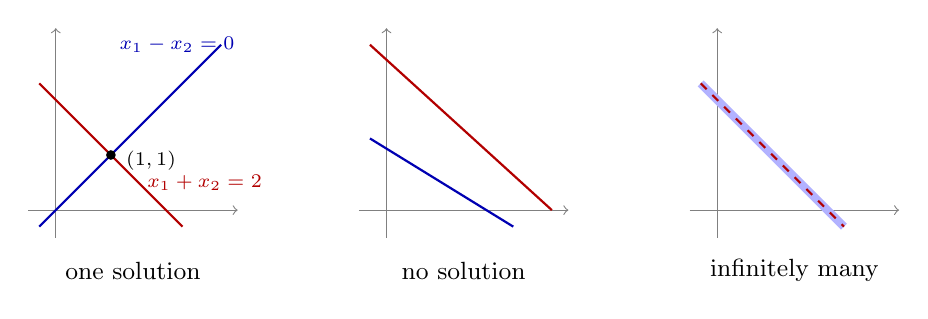
\begin{tikzpicture}[scale=0.7]
  \foreach \s/\title in {0/{one solution},6/{no solution},12/{infinitely many}} {
    \begin{scope}[xshift=\s cm]
      \draw[->,gray] (-0.5,0) -- (3.3,0); \draw[->,gray] (0,-0.5) -- (0,3.3);
      \node[font=\small] at (1.4,-1.1) {\title};
    \end{scope}
  }
  \draw[thick,blue!70!black] (-0.3,-0.3) -- (3,3);
  \draw[thick,red!70!black] (-0.3,2.3) -- (2.3,-0.3);
  \fill (1,1) circle (2.5pt);
  \node[font=\scriptsize,right] at (1.1,0.9) {$(1,1)$};
  \node[font=\scriptsize,blue!70!black] at (2.2,3.0) {$x_1 - x_2 = 0$};
  \node[font=\scriptsize,red!70!black] at (2.7,0.5) {$x_1 + x_2 = 2$};
  \begin{scope}[xshift=6cm]
    \draw[thick,blue!70!black] (-0.3,1.3) -- (2.3,-0.3);
    \draw[thick,red!70!black] (-0.3,3.0) -- (3,0);
  \end{scope}
  \begin{scope}[xshift=12cm]
    \draw[line width=3pt,blue!30] (-0.3,2.3) -- (2.3,-0.3);
    \draw[thick,red!70!black,dashed] (-0.3,2.3) -- (2.3,-0.3);
  \end{scope}
\end{tikzpicture}
\end{center}

\section{Augmented matrices and row operations}

We record only the numbers. The \emph{coefficient matrix} is $A=[a_{ij}]$ ($m\times n$) and the
\emph{augmented matrix} is $[A\mid\vec b]$:
\[
  \left[\begin{array}{cccc|c}
    a_{11} & a_{12} & \cdots & a_{1n} & b_1\\
    \vdots & & & \vdots & \vdots\\
    a_{m1} & a_{m2} & \cdots & a_{mn} & b_m
  \end{array}\right].
\]

\begin{definition}[Elementary row operations]
\begin{enumerate}
  \item Multiply a row by a \emph{non-zero} scalar: $cR_i$, $c\ne0$.
  \item Add a multiple of one row to another: $R_i + cR_j$ ($i\ne j$).
  \item Swap two rows: $R_i\leftrightarrow R_j$.
\end{enumerate}
Two matrices are \emph{row equivalent} if one can be obtained from the other by a finite
sequence of elementary row operations.
\end{definition}

\begin{theorem}
If $[A\mid\vec b]$ and $[C\mid\vec d]$ are row equivalent, the corresponding systems have the same
solution set.
\end{theorem}
\begin{proof}[Proof sketch]
Any solution of the original equations satisfies the new equations (they are combinations of
the old ones). Each row operation is reversible by an operation of the same type
($\frac1cR_i$, $R_i-cR_j$, $R_i\leftrightarrow R_j$), so the converse holds too.
\end{proof}

\section{Row echelon form and reduced row echelon form}

\begin{definition}[REF and RREF]
A matrix is in \emph{row echelon form} (REF) if
\begin{enumerate}
  \item all zero rows are at the bottom, and
  \item the first non-zero entry (the \emph{leading entry}) of each non-zero row is strictly to the
        right of the leading entry of the row above.
\end{enumerate}
It is in \emph{reduced row echelon form} (RREF) if additionally
\begin{enumerate}[resume]
  \item every leading entry is $1$ (a \emph{leading one}), and
  \item each leading one is the only non-zero entry in its column.
\end{enumerate}
\end{definition}

\begin{theorem}
Every matrix is row equivalent to a matrix in REF, and to a \emph{unique} matrix in RREF.
\end{theorem}

Uniqueness of the RREF is what makes the next definition meaningful (an REF is not unique, but
the positions of its leading entries are).

\begin{definition}[Rank, pivots]
The \emph{rank} of $A$, $\rank A$, is the number of leading ones in the RREF of $A$ (equivalently,
the number of leading entries in any REF). Columns containing leading entries are \emph{pivot
columns}; in a system, the variables of pivot columns are \emph{leading variables} and the rest
are \emph{free variables}.
\end{definition}

\section{Gaussian and Gauss--Jordan elimination}

\begin{important}[Algorithm]
\textbf{Gaussian elimination}: row reduce $[A\mid\vec b]$ to REF working left to right, creating
zeros \emph{below} each leading entry; then solve by back-substitution.
\textbf{Gauss--Jordan elimination}: continue to RREF (zeros above and below every leading one),
then read the solution off directly.
\end{important}

\begin{example}[A unique solution]
Solve $x_1+x_2+x_3=6$, $2x_1+3x_2+x_3=11$, $x_1-x_2+2x_3=5$.
\[
\left[\begin{array}{ccc|c} 1&1&1&6\\ 2&3&1&11\\ 1&-1&2&5\end{array}\right]
\xrightarrow{\substack{R_2-2R_1\\R_3-R_1}}
\left[\begin{array}{ccc|c} 1&1&1&6\\ 0&1&-1&-1\\ 0&-2&1&-1\end{array}\right]
\xrightarrow{R_3+2R_2}
\left[\begin{array}{ccc|c} 1&1&1&6\\ 0&1&-1&-1\\ 0&0&-1&-3\end{array}\right]
\]
This is an REF. Continuing to RREF:
\[
\xrightarrow{-R_3}
\left[\begin{array}{ccc|c} 1&1&1&6\\ 0&1&-1&-1\\ 0&0&1&3\end{array}\right]
\xrightarrow{\substack{R_1-R_3\\R_2+R_3}}
\left[\begin{array}{ccc|c} 1&1&0&3\\ 0&1&0&2\\ 0&0&1&3\end{array}\right]
\xrightarrow{R_1-R_2}
\left[\begin{array}{ccc|c} 1&0&0&1\\ 0&1&0&2\\ 0&0&1&3\end{array}\right].
\]
The unique solution is $\vec x=(1,2,3)$. Check in the second equation: $2+6+3=11$.
\end{example}

\begin{example}[Infinitely many solutions; parametric vector form]
Solve the system with augmented matrix
\[
\left[\begin{array}{cccc|c} 1&2&0&1&3\\ 2&4&1&4&8\\ 1&2&1&3&5\end{array}\right]
\xrightarrow{\substack{R_2-2R_1\\R_3-R_1}}
\left[\begin{array}{cccc|c} 1&2&0&1&3\\ 0&0&1&2&2\\ 0&0&1&2&2\end{array}\right]
\xrightarrow{R_3-R_2}
\left[\begin{array}{cccc|c} 1&2&0&1&3\\ 0&0&1&2&2\\ 0&0&0&0&0\end{array}\right].
\]
This is already RREF. Leading variables: $x_1,x_3$; free variables: $x_2=s$, $x_4=t$. Then
$x_1 = 3-2s-t$, $x_3 = 2-2t$, and the solution set in \emph{parametric vector form} is
\[
  \vec x = \begin{bmatrix}3\\0\\2\\0\end{bmatrix}
         + s\begin{bmatrix}-2\\1\\0\\0\end{bmatrix}
         + t\begin{bmatrix}-1\\0\\-2\\1\end{bmatrix},\qquad s,t\in\R .
\]
Check with the third original equation: $(3-2s-t)+2s+(2-2t)+3t = 5$. Geometrically this is a
plane in $\R^4$ not through the origin.
\end{example}

\begin{example}[Depending on parameters]
For which $k,m$ is the system with augmented matrix below inconsistent / uniquely solvable /
infinitely solvable?
\[
\left[\begin{array}{ccc|c} 1&1&1&1\\ 1&2&3&2\\ 1&3&k&m\end{array}\right]
\xrightarrow{\substack{R_2-R_1\\R_3-R_1}}
\left[\begin{array}{ccc|c} 1&1&1&1\\ 0&1&2&1\\ 0&2&k-1&m-1\end{array}\right]
\xrightarrow{R_3-2R_2}
\left[\begin{array}{ccc|c} 1&1&1&1\\ 0&1&2&1\\ 0&0&k-5&m-3\end{array}\right].
\]
\begin{itemize}
  \item $k\ne5$: three leading entries in the coefficient part, so a unique solution.
  \item $k=5$, $m\ne3$: the last row reads $0=m-3\neq 0$; inconsistent.
  \item $k=5$, $m=3$: the last row is zero, $x_3$ is free; infinitely many solutions.
\end{itemize}
\end{example}

\begin{important}[Pitfall]
Do not perform two operations ``at once'' that use a row being changed in the same step (e.g.
$R_1-R_2$ and $R_2-R_1$ simultaneously); this can destroy information. Also, $R_i\to cR_i+R_j$ is
fine only if $c\ne 0$; ``$R_i \to 0R_i + R_j$'' is not a row operation.
\end{important}

\section{Rank and the structure of solution sets}

\begin{theorem}[System-Rank Theorem]
Let $A$ be $m\times n$.
\begin{enumerate}
  \item $[A\mid\vec b]$ is inconsistent iff its RREF has a row $[0\ \cdots\ 0\mid 1]$, i.e. iff
        $\rank A < \rank[A\mid\vec b]$.
  \item If the system is consistent, the solution set has $n-\rank A$ free parameters.
  \item $A\vec x=\vec b$ is consistent for \emph{every} $\vec b\in\R^m$ iff $\rank A = m$.
\end{enumerate}
\end{theorem}
\begin{proof}[Proof sketch]
(1) and (2) are read off the RREF: each non-pivot column of $A$ gives one free variable.
For (3): if $\rank A=m$, every row of the RREF of $A$ has a leading one, so a bad row
$[0\cdots0\mid 1]$ cannot occur. If $\rank A<m$, the RREF $R$ of $A$ has a zero row; start from
$[R\mid\vec e_m]$ and reverse the row operations to get a $\vec b$ for which the system is
inconsistent.
\end{proof}

\begin{corollary}
Since $\rank A\le\min(m,n)$: a set of $k$ vectors in $\R^n$ with $k>n$ is linearly dependent, and a
set of $k<n$ vectors cannot span $\R^n$. Hence every basis of $\R^n$ has exactly $n$ vectors.
\end{corollary}
\begin{proof}
Put the vectors as columns of an $n\times k$ matrix $A$. Independence means $A\vec c=\vec 0$ has
only the trivial solution, i.e. $k-\rank A=0$; but $\rank A\le n<k$. Spanning means $A\vec c=\vec b$
is consistent for all $\vec b$, i.e. $\rank A = n$; but $\rank A\le k<n$.
\end{proof}

\begin{important}[Using row reduction for span and independence]
For $\vec v_1,\dots,\vec v_k\in\R^n$ and $A=[\vec v_1\ \cdots\ \vec v_k]$:
\begin{itemize}
  \item $\vec b\in\Span\{\vec v_i\}$ iff $[A\mid\vec b]$ is consistent;
  \item $\{\vec v_i\}$ spans $\R^n$ iff $\rank A = n$;
  \item $\{\vec v_i\}$ is linearly independent iff $\rank A = k$.
\end{itemize}
\end{important}

\section{Homogeneous systems}

\begin{definition}
A system is \emph{homogeneous} if all right-hand sides are $0$: $A\vec x=\vec 0$. It is always
consistent, since $\vec x=\vec 0$ (the \emph{trivial solution}) works.
\end{definition}

\begin{theorem}
The solution set of a homogeneous system in $n$ variables is a subspace of $\R^n$ (the
\emph{solution space}). Moreover, if $\vec x_p$ is any one solution of $A\vec x=\vec b$, then the
full solution set of $A\vec x=\vec b$ is $\{\vec x_p+\vec x_h : A\vec x_h=\vec 0\}$.
\end{theorem}
\begin{proof}
If $\vec x,\vec y$ solve the homogeneous system then each equation gives
$\sum_j a_{ij}(x_j+y_j)=0+0$ and $\sum_ja_{ij}(cx_j)=c\cdot0$. For the second claim, if
$A\vec x=\vec b$ then $\vec x-\vec x_p$ solves the homogeneous system, and conversely
$A(\vec x_p+\vec x_h)=\vec b+\vec 0$.
\end{proof}

So the solution set of $A\vec x = \vec b$ is the solution space of $A\vec x=\vec 0$ shifted by
any one particular solution:
\begin{center}
\begin{tikzpicture}[scale=0.9,>={Stealth}]
  \draw[->,gray] (-2.5,0) -- (4,0); \draw[->,gray] (0,-1.2) -- (0,3.4);
  \draw[thick,blue!70!black] (-2.4,-0.8) -- (3.6,1.2) node[right] {$\{\vec x : A\vec x = \vec 0\}$};
  \draw[thick,red!70!black] (-2.4,1.2) -- (3.6,3.2) node[right] {$\{\vec x : A\vec x = \vec b\}$};
  \draw[->,thick] (0,0) -- (0.6,2.2) node[left] {$\vec x_p$};
  \draw[->,thick,blue!70!black] (0,0) -- (1.8,0.6) node[below right] {$\vec x_h$};
  \draw[->,thick,red!70!black] (0,0) -- (2.4,2.8) node[above left] {$\vec x_p + \vec x_h$};
  \draw[dashed] (0.6,2.2) -- (2.4,2.8) (1.8,0.6) -- (2.4,2.8);
\end{tikzpicture}
\end{center}

In the infinitely-many-solutions example above, $\vec x_p=(3,0,2,0)$ and the homogeneous
solution space is $\Span\{(-2,1,0,0),(-1,0,-2,1)\}$; the spanning vectors produced by the
free variables are automatically linearly independent (look at the free-variable positions).

\begin{example}
Find a basis for the solution space of $x_1-x_2+2x_3=0$, $2x_1-x_2+x_3=0$.
\[
\left[\begin{array}{ccc|c} 1&-1&2&0\\ 2&-1&1&0\end{array}\right]
\xrightarrow{R_2-2R_1}
\left[\begin{array}{ccc|c} 1&-1&2&0\\ 0&1&-3&0\end{array}\right]
\xrightarrow{R_1+R_2}
\left[\begin{array}{ccc|c} 1&0&-1&0\\ 0&1&-3&0\end{array}\right].
\]
With $x_3=t$: $\vec x = t(1,3,1)$, so $\{(1,3,1)\}$ is a basis. Check: $1-3+2=0$, $2-3+1=0$.
\end{example}

\section*{Summary}
\begin{itemize}
  \item A linear system has $0$, $1$ or infinitely many solutions.
  \item Elementary row operations preserve the solution set; reduce to REF (Gaussian) or RREF
        (Gauss--Jordan). The RREF is unique; $\rank A$ = number of leading ones.
  \item Inconsistent iff a row $[0\cdots0\mid1]$ appears; otherwise $n-\rank A$ parameters.
  \item $A\vec x=\vec b$ is solvable for all $\vec b$ iff $\rank A=m$; columns independent iff
        $\rank A = n$.
  \item Homogeneous solution sets are subspaces; general solution = particular + homogeneous.
\end{itemize}
